\chapter{Yuanfudao system}
\label{chap:yuanfudao}
On the 2018 Semeval Task \textit{Machine comprehension using commonsense knowledge} competition the \texttt{Yuanfudao} \cite{Wang:2018} system reached second place with $83.95\%$ accuracy on the test data.

% Yuanfudao introduction
\section{The original system}

The \texttt{Yuanfudao} system implements a Three-way Attentive Network (TriAN), an ensemble of three LSTMs augmented with various attention mechanisms, to model for each question interactions between question, possible answers, and the passage that may or may not contain the correct answer to the question.

The system was implemented using python programming language and the \texttt{pytorch} package for the implementation of the neural network. The source code is available on Github\footnote{\url{https://github.com/intfloat/commonsense-rc}}.

\subsection{Parameters}

The \texttt{Yuanfudao} system has these following command line arguments:
\begin{itemize}
	\item \textbf{GPU}: the training of the system can be done on GPU which is much faster than training it on CPU
	\item \textbf{using cuda}: \texttt{pytorch} can support CUDA for parallelization. The system uses CUDA by default.
	\item \textbf{optimizer}: the optimizer function can be adamax (default) or SGD
	\item \textbf{RNN type}: the RNN used by the system can be LSTM or GRU
	\item \textbf{dropout rate}: there are separate dropout rates for embeddings and RNNs
	\item \textbf{embedding dimension}: each embedding dimension in the system can be manually set
	\item \textbf{gradient clipping}: the gradient clipping threshold can be set
	\item \textbf{epoch}
	\item \textbf{learning rate}
	\item \textbf{batch size}
	\item \textbf{random seed}
	\item other parameters related to input handling, RNN settings and testing
\end{itemize}
You can read about the deep learning related arguments and their functions in Chapter \ref{chap:deep}.

% Yuanfudao preprocess

\subsection{Preprocessing}
This system processes the input data as follows:

\begin{enumerate}
	\item Using the \texttt{spacy} package's tokenizer function it generates the part of speech (pos) tag, named entity recognition (ner) tag and the lemma for each word in the passage, and the pos tags of the questions.
	\item It assigns a number representation and an offset for each word in the passage, questions and answers.
	\item It also saves the ids of the passages, questions and answers and whether the answer was correct.
	\item The preprocessor finds the words and lemmas in the questions and answers, that also occurred in the passage's word and lemma list. 
	\item It stores each word's frequency using the \texttt{wikiwords} library.
	\item It  establishes the \textit{ConceptNet} relation between the words of the passage and question and also between the words of the passage and answer.
	\item The preprocessor saves all this data to their respective json files.
\end{enumerate}

% Conceptnet

The \textit{ConceptNet} is a major part of the \texttt{Yuanfudao} system, as it was shown in the original paper \cite{Wang:2018}. This metric is to show the possible relationship between two words. These relations could be "RelatedTo", "IsA", "Synonym", "PartOf" etc. The preprocessor compares the words in the passage with the words in the "query" (question or answer) and stores only one of the matches per word, if there were any.

An overview of the original system is reproduced in Figure~\ref{fig:dnn}.
\begin{figure}[h!]
	\centering
	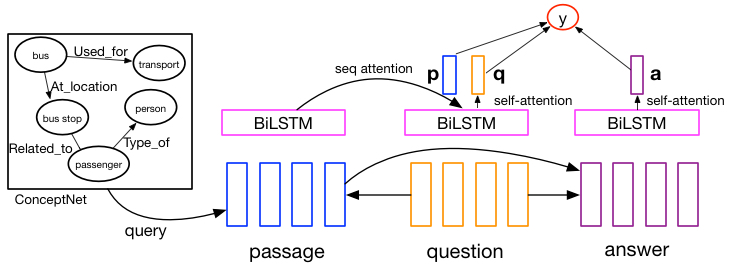
\includegraphics[scale=0.5]{TriAN.jpg}
	\caption{Structure of the original network \cite{Wang:2018}}
	\label{fig:dnn}
\end{figure}

This system is a deep learning neural network consisting of embeddings, recurrent neural networks and attention mechanisms.

% System description

\subsection{System description}

First the inputs generated in the preprocessing phase go through three embedding layers, each corresponding to the passage, question and answer respectively. There are also pos-embedding, ner-embedding and rel-embedding layers. The pos embedding gets the passage's and the question's pos tags as its input, the ner embedding layer gets the passage's ner tags and the relation embedding gets the relationship vectors generated using the \textit{ConceptNet}. This input embedding layer is shown in Figure~\ref{fig:embedding}.
\begin{figure}[h!]
	\centering
	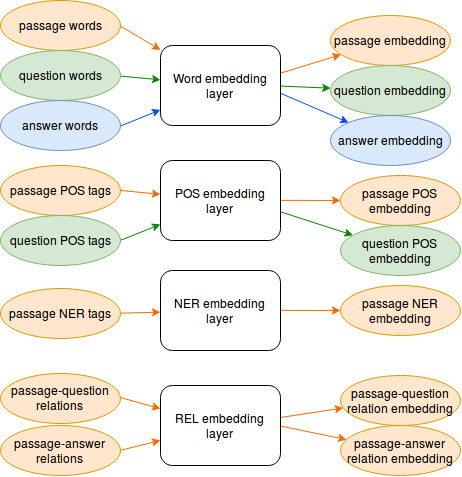
\includegraphics[scale=0.5]{TriAN_embeddings.jpg}
	\caption{Structure of the input embedding layers.}
	\label{fig:embedding}
\end{figure}

The word embeddings' outputs are paired up (passage-question, answer-question, answer-passage) and go through a so called \textit{sequence attention matching layer}.
The \textit{sequence attention matching layer} at its core uses the bmm function in \texttt{pytorch} which performs a batch matrix-matrix product of the input matrices.
This way it "matches" the two inputs together. This is shown in Figure~\ref{fig:attention_match}.
\begin{figure}[h!]
	\centering
	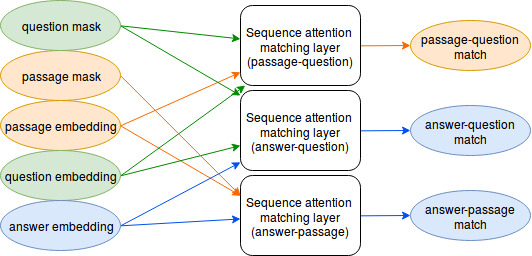
\includegraphics[scale=0.5]{TriAN_attention_match.jpg}
	\caption{Structure of the \textit{sequence attention matching layers}.}
	\label{fig:attention_match}
\end{figure}

The system uses dropouts after the embedding and \textit{sequence attention matching layer} layers to avoid over-fitting.

These layers are followed by three \textit{stacked bidirectional RNN layer}, each corresponding to the passage, question and answer respectively. It differs from the standard bidirectional RNN layer in one aspect: it can concatenate the hidden states of the RNN. By default the type of the RNN is LSTM, but it can also be GRU. Their inputs are sort of self explanatory. The passage's \textit{stacked bidirectional RNN layer} gets the passage's word embedding layer, the output of the \textit{sequence attention matching layer} for the passage-question input pair, the passage's pos and ner embedding layers, the word frequency tensor created with the \texttt{wikiword} library, and the two relation embedding layer's output. The question's \textit{stacked bidirectional RNN layer} expects the question's word and pos embedding outputs on its input. The answer's \textit{stacked bidirectional RNN layer's} inputs are the answer's word embedding output and  the output of the \textit{sequence attention matching layer} for the answer-question and the answer-question input pairs. These RNN layers are shown in the Figure~\ref{fig:rnn}.
\begin{figure}[h!]
	\centering
	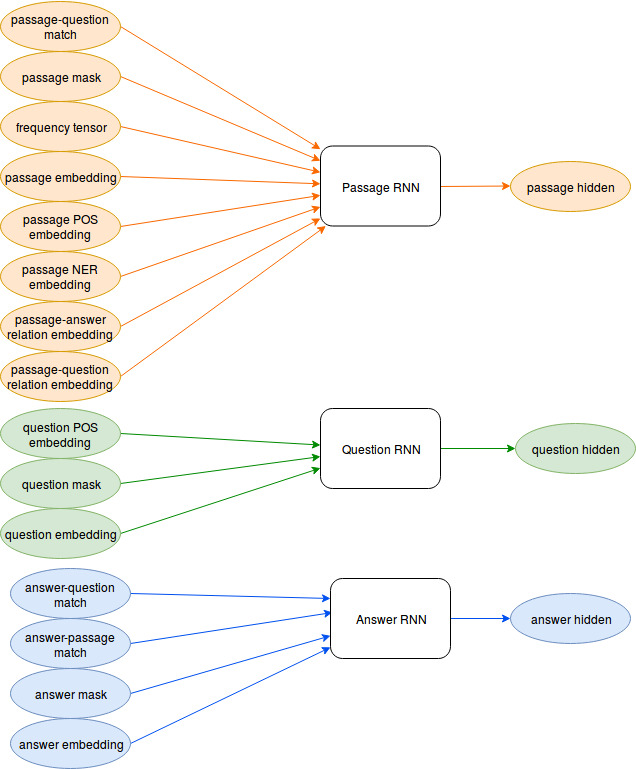
\includegraphics[scale=0.4]{TriAN_rnn.jpg}
	\caption{Structure of the \textit{stacked bidirectional RNN layers}.}
	\label{fig:rnn}
\end{figure}
This layer implicitly uses a dropout rate for regularization.

The question's and the answer's \textit{stacked bidirectional RNN layer's} outputs are used in two \textit{linear sequence attention layers}, or better known as \textit{self-attention layers over a sequence} for the question and the answer respectively. This layer is basically a linear layer slightly modified, so the infinite outputs are masked and it uses a softmax function at its output.

The passage's \textit{stacked bidirectional RNN layer's} output is used differently. The system passes it and the question's \textit{stacked bidirectional RNN layer's} output to a \textit{bilinear sequence attention layer}, which is similarly to the \textit{sequence attention matching layer} uses the bmm function as its core function.

The two \textit{linear sequence attention layer's} and the \textit{bilinear sequence attention layer's} output is passed through a weighted averaging function with their respective \textit{stacked bidirectional RNN layer's} output. This part of the network is shown in Figure~\ref{fig:sequence_attention}.
\begin{figure}[h!]
	\centering
	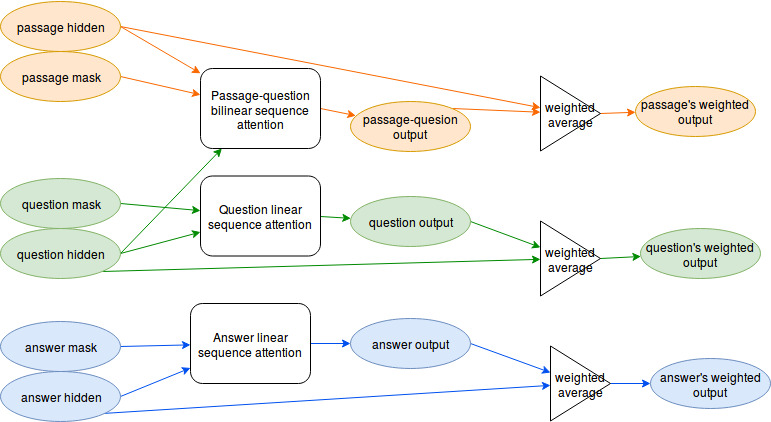
\includegraphics[scale=0.5]{TriAN_sequence_attention.jpg}
	\caption{Structure of the sequence attention layer\\and the following weighted average function.}
	\label{fig:sequence_attention}
\end{figure}

The averaged passage output is passed though a \textit{linear feed forward layer} than multiplied by the answer's averaged output. The question's averaged output is passed though an other \textit{linear feed forward layer} than multiplied by the answer's averaged output. At the end its all summed and sigmoid function used at its output. The output in this case is whether the answer was correct to the given question or not. This last section is at Figure~\ref{fig:output}.
\begin{figure}[!htb]
	\centering
	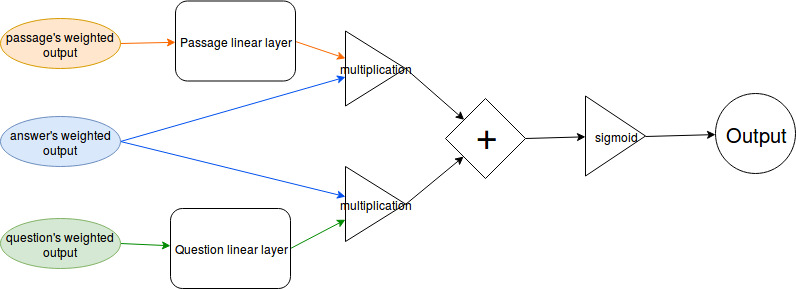
\includegraphics[scale=0.5]{TriAN_output.jpg}
	\caption{Structure of the output of the network.}
	\label{fig:output}
\end{figure}

\subsection{Learning curve}
\begin{minipage}{\linewidth}
Without the recommended pretraining (Figure~\ref{fig:learning_curve}):
\begin{itemize}
	\item Max dev accuracy: $82.7\%$ reached in the 26th epoch
	\item Train accuracy: $97.7\%$ reached in the 26th epoch
	\item Max train accuracy: $99.8\%$ reached in the 50th epoch
	\item Last dev accuracy: $81.9\%$
	\item Average dev accuracy after ten epochs: $81.9\%$
\end{itemize}
\end{minipage}
\begin{figure}[!htb]
	\centering
	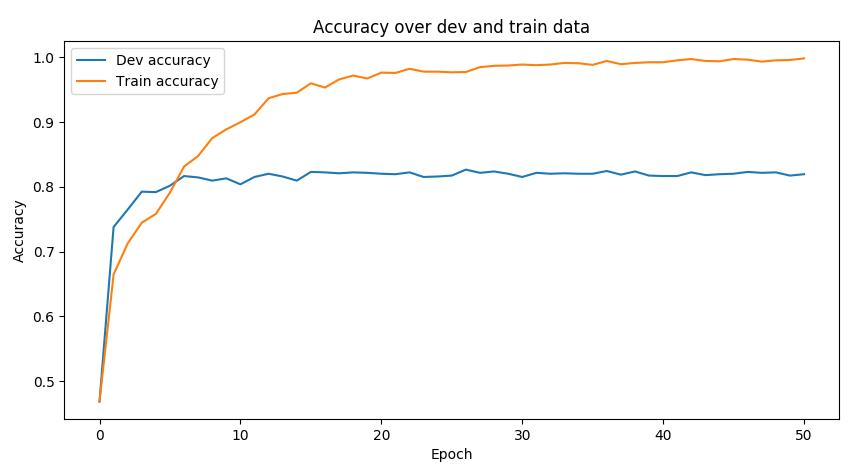
\includegraphics[scale=0.5]{learning_curve.jpg}
	\caption{Learning curve without pretraining.}
	\label{fig:learning_curve}
\end{figure}

\begin{minipage}{\linewidth}
With the recommended pretraining(Figure~\ref{fig:learning_curve2}):
\begin{itemize}
	\item Max dev accuracy: $82.5\%$ reached in the 38th epoch
	\item Train accuracy: $99\%$ reached in the 38th epoch
	\item Max train accuracy: $99.7\%$ reached in the 50th epoch
	\item Last dev accuracy: $82.2\%$
	\item Average dev accuracy after ten epochs: $81.9\%$
\end{itemize}
\end{minipage}
\begin{figure}[!htb]
	\centering
	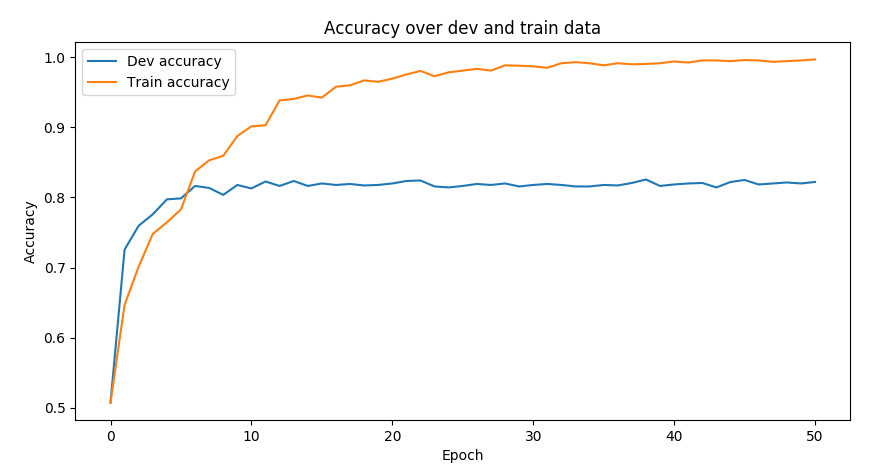
\includegraphics[scale=0.5]{learning_curve2.jpg}
	\caption{Learning curve with pretraining.}
	\label{fig:learning_curve2}
\end{figure}

As you can see there is no significant difference between the learning curve with or without pretraining.

\section{Modifications}
Our modifications are available on Github\footnote{\url{https://github.com/GKingA/commonsense-rc}}.

We modified the preprocessing part of the system to incorporate the similarity calculating method from Chapter ~\ref{chap:4lang}. The most straightforward way of incorporating our metric into the system is by creating vectors similar to those representing \textit{ConceptNet} relations between words of a passage and words in each answer candidate. Since these vectors represent
word-to-word relationships, we measure the support between pairs of \texttt{4lang} definition graphs, and for each word in the passage we take the maximum support score over all words of the answer candidate. Elements of a vector for a passage $P$ and a possible answer $A$ are hence defined as:

\[S^{(P, A)}_i = \max_{A_j \in A} S(P_i, A_j)\]

Elements of a vector for a passage $P$ and a question $Q$ are defined as:

\[S^{(P, Q)}_i = \max_{Q_j \in Q} S(P_i, Q_j)\]

Elements of a vector for a question $Q$ and an answer $A$ are defined as:

\[S^{(Q, A)}_i = \max_{A_j \in A} S(Q_i, A_j)\]

We used these new input vectors as the input of a new \texttt{4lang} embedding layer that functions similarly to the other embedding layers. It is shown at Figure~\ref{fig:4lang_embedding}. The input of this layer is 101 dimensional, since the similarities are on a scale to 0 to 100.

\begin{figure}[h!]
	\centering
	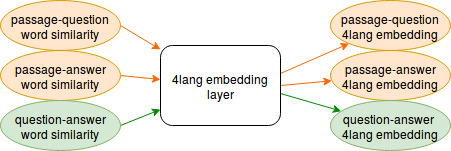
\includegraphics[scale=0.5]{4lang_embedding.jpg}
	\caption{\texttt{4lang} embedding layer.}
	\label{fig:4lang_embedding}
\end{figure}

The outputs of this layer is passed to the RNN layers. This is depicted at Figure~\ref{fig:rnn_4lang}.

\begin{figure}[h!]
	\centering
	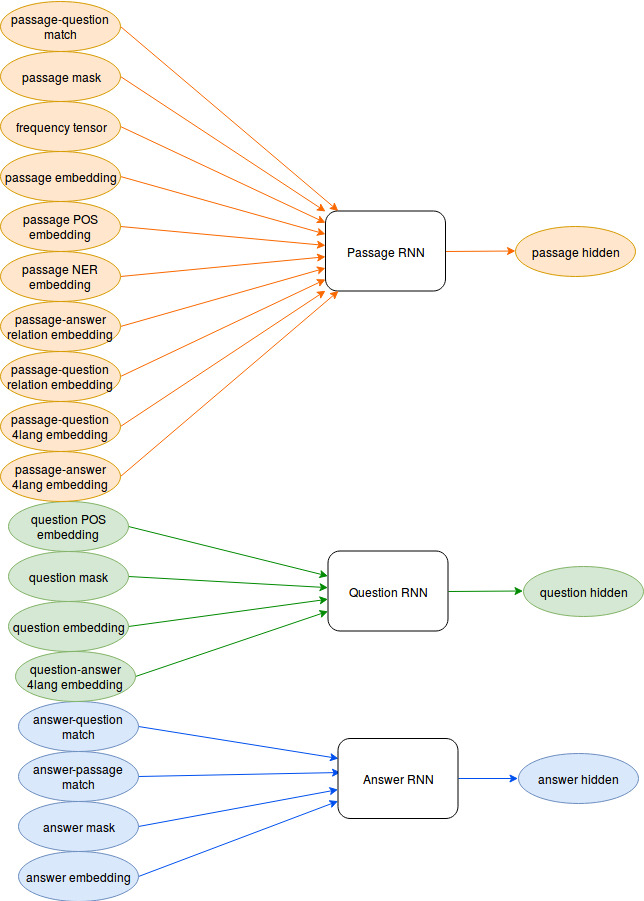
\includegraphics[scale=0.4]{TriAN_rnn_with_4lang.jpg}
	\caption{Structure of the modified \textit{stacked bidirectional RNN layers}.}
	\label{fig:rnn_4lang}
\end{figure}

Since we also wanted to see how the system changes if we replace \textit{ConceptNet} relations with our metric, we also trained systems without \textit{ConceptNet} rel embeddings.

\FloatBarrier

\section{The results}
The original \texttt{Yuanfudao} \cite{Wang:2018} publication said its system was able to reach $83.95\%$ accuracy on the test data. We were only able to reproduce a $80.3\%$ accuracy on the test set and $82.5\%$ on the development set with the recommended pretraining on the \texttt{RACE} \cite{Lai:2017} dataset. We will take these results as our bases of the comparison.

\begin{table}[h!]
	\centering
	\begin{tabular}{ | l | c | r | }
		\hline
		model & dev & test \\ \hline \hline
		pretrained TriAN, no ConceptNet & 83.7\% & 81.9\% \\ \hline
		pretrained TriAN, with ConceptNet & 82.5\% & 80.3\% \\ \hline
		pretrained TriAN, with 4lang & 84.2\% & 81.5\% \\ \hline
		\textbf{pretrained TriAN, with both} & \textbf{83.4\%} & \textbf{82.9\%} \\ \hline
		TriAN, no ConceptNet & 82.8\% & 80.2\% \\ \hline
		TriAN, with ConceptNet & 82.7\% & 80.5\% \\ \hline
		TriAN, with 4lang & 83.2\% & 80.9\% \\ \hline
		TriAN, with both & 83.1\% & 80.8\% \\ \hline
	\end{tabular}
	\caption{Effect of \texttt{4lang} and \texttt{ConceptNet} on results}
	\label{tabl:res}
\end{table}